\newcommand{\bA}{{\mathbf{D}}}
\newcommand{\bB}{{\mathbf{B}}}
\newcommand{\bC}{{\mathbf{P}}}
\newcommand{\bP}{{\mathbf{P}}}
\newcommand{\bF}{{\mathbf{F}}}
\newcommand{\bL}{{\mathbf{L}}}
\newcommand{\ba}{{\mathbf{d}}}
\newcommand{\bp}{{\mathbf{p}}}
\newcommand{\bs}{{\mathbf{s}}}
\newcommand{\by}{{\mathbf{y}}}

\subsection{Problem definition}\label{ss:problem_definition}
Given an RNA sequence $\bs$ probed at $N$ nucleotides, assume that we carry out the chemical structure probing of this sequence using $M$ different treatments, each of which is run in a separate capillary lane. Assume that the fluorescence intensity of each capillary is measured over $K$ time points. We define a \emph{profile} (also called a \emph{trace}) as the sequence of intensity values from a capillary. \hilight{For any particular profile, the reactivity of each nucleotide to the chemical reagent is represented at a specific location in the series of intensity values, and $N$ such locations are sequentially spread throughout the entire profile. All profiles are assumed to be well aligned using the procedure described in~\citet{Yoon2011} such that each nucleotide corresponds to the same location across all profiles. The entire CE measurement can then be arranged in a $K \times M$ matrix $\bA$.} Normally, $N \ll K$, i.e. each electrophoretic profile is finely sampled in time. Based on the characteristic of the chemical agent used in each treatment and the secondary structure computationally inferred from the input sequence, we can predict the fluorescence intensity at each position of $\bs$ for each of $M$ treatments. This prediction can be arranged in a $N \times M$ matrix $\bC$ called the \emph{prediction matrix} (see below).

The problem of band annotation is \hilight{therefore} formulated as selecting $N$ out of the $K$ rows of $\bA$ using the information in $\bC$ in such a way that a certain objective is optimized over all possible ${K \choose N}$ possibilities. The selected $N$ points map to the locations of the nucleotides of the sequence $\bs$ in the CE measurement \hilight{(see Supplemental Fig. S1)}.

The input of the proposed method consists of the following:
\begin{itemize}
\item $\bA \in \mathbb{R}^{K \times M}$: the fluorescence intensity matrix
\item $\bC \in \{0,1\}^{N \times M}$: the prediction matrix
\item $\bs \in \{\mathtt{A}, \mathtt{C}, \mathtt{G}, \mathtt{U}\}^N$: the nucleotide sequence
\end{itemize}
and the output is an array $\by \in \mathbb{Z}_+^N$ representing $N$ band locations selected out of $K$.




\subsection{Prediction matrix construction}\label{ss:pred_mat}
Figure~\ref{f:pred-mat}(a) defines the expected reactivity of each type of nucleotide to chemical reagents used for chemical probing under the (un)paired condition. The value of one means that the nucleotide is reactive to the reagent, whereas zero indicates no reactivity. For instance,  the DMS chemical modifies \texttt{A} and \texttt{C} but not \texttt{U} and \texttt{G}, and the entries for \texttt{A} and \texttt{C} are one, while those for \texttt{U} and \texttt{G} are zero. We allow the use of numerous chemical probing strategies: dimethyl sulfate alkylation [DMS], carbodiimide modification [CMCT], and `others' that can produce bands at all locations, including $2^{\prime}$-OH acylation [the SHAPE strategy] \citep{Kladwang2014}. \hilight{We also allow input of a secondary structure in dot-parentheses notation.} Nucleotides forming base pairs are not expected to show bands in DMS, CMCT, SHAPE, and other structure mapping profiles. Sequencing experiments that terminate reverse transcription of the RNA with ddNTP incorporation produce bands after nucleotides complementary to the terminating nucleotide. Based on this information, we construct the prediction matrix $\bP$ that stores the expected chemical reactivity for individual residues. The element $p_{ij} \in \bP$ indicates such reactivity information of residue $i$ to reagent $j$.

%

Figure~\ref{f:pred-mat}(b) shows an example RNA sequence with its secondary structure. Figure~\ref{f:pred-mat}(c) shows the corresponding prediction matrix $\bP$.


\subsection{Initialization of candidate peaks from profiles}\label{ss:preproc}
\hilight{The first step is to locate prominent peaks on each profile (each column of $\bA$). As discussed in Section~\ref{ss:problem_definition}, peaks in CE profiles are the locations where significant reactivities are observed, implying that bands are more likely to exists at the same position. Thus, these peaks are matched with bands afterwards.} (Here and below, `peak' refers to a local maximum in each profile, \hilight{of which there may be many}; whereas `bands' refers to the desired $N$ band locations.) Let $\ba_j$ be the $j$-th column vector of $\bA, 1 \le j \le M$. Briefly, the following procedure is executed.
%
\begin{enumerate}
\item Select candidates for the peaks in $\ba_j$ that can be mapped into elements of the sequence $\bs$. These peaks are selected to satisfy the following conditions. First, a peak $\ba_j(k)$ must have a higher intensity (a fundamental property of a peak) than those of its neighbors, $\ba_j(k-1)$ and $\ba_j(k+1)$. Second, a peak must be with a significant curvature which can be measured by the second derivative of time series; since the time series given are discrete, the curvature is estimated as belows:
%
\begin{equation}\label{e:gamma}
\Gamma = \Delta^- - \Delta^+
\end{equation}
%
where
%
\begin{eqnarray}
\Delta^- = \max( \ba_j(k)-\ba_j(k-1), {{(\ba_j(k)-\ba_j(k-2))}\over{2}}) \nonumber \\
\Delta^+ = \min( \ba_j(k+1)-\ba_j(k), {{(\ba_j(k+2)-\ba_j(k))}\over{2}}) \nonumber
\end{eqnarray}
%
The $\Delta^-$ and $\Delta^+$ in (\ref{e:gamma}) approximate the slope of left and right side of peak respectively, and $\Gamma$ is the difference between them; thus, the magnitude of $\Gamma$ represents how abruptly the curve has turned from upwards to downwards. Now we choose $N^\textrm{peak}_j$ peaks with highest $\Gamma$ from the points satisfying the first condition, \hilight{where $N^\textrm{peak}_j$ is set proportionally to the number nucleotides reactive to the chemical agent used for the $j$-th profile (\ie the number of ones on the $j$-th column of $\bP$)}. Call these candidate peak locations $A^i$ $(1 \le i \le N^\textrm{peak}_j$).

\item In preparation for the sampling scheme and scorefunction computation below, estimate the ideal separation between bands based on the remaining peak locations: \hilight{$\rho \triangleq (\max\limits_{j}{k_j^r} - \min\limits_{j}{k_j^f}) / (N-1)$, where $k_j^f$ and $k_j^r$ are the locations of the foremost peak and the rearmost peak respectively on the $j$-th profile.}% The ideal separation calculated here is used when shifting the window in dynamic programming.

%\item In order to remove the influence of noise that every $\ba_j$ has in common near the end of the time series, eliminate a portion of tailing peaks as follows: Identify 5 tailing peaks and select one with the hightest intensity among them. Denote $i_j$ be the time index of this peak $(1 \le i_j \le K)$. Let $i^*=\max_{1 \le j \le M} i_j$. For each $\ba_j$, remove all peaks appearing after $i^*$.
\item In preparation for the scorefunction computation below, construct a matrix based on these candidate peak locations called the \emph{bonus matrix} $\bB \in \mathbb{Z}^{K \times M}$. Let $\bar{\Gamma}$ be the mean value of $\Gamma_i$ of the candidate peaks. Initialize $\bB$ to all zero. At each peak $A^i$, we apply a uniform bonus, supplemented by a stronger bonus at sharp peaks: \hilight{$\bB(A^i,j) = \bar{\Gamma}/2 + \Gamma_i$}.

\end{enumerate}




%%%%%%%%%%%%%%%%%%%%%%%%%%%%%%%%%%%%%%%%%%%%%%%%%%%%%%%%%%%%%%%%%%%%%%%%%%%%%%%%
% Prediction Matrix
%%%%%%%%%%%%%%%%%%%%%%%%%%%%%%%%%%%%%%%%%%%%%%%%%%%%%%%%%%%%%%%%%%%%%%%%%%%%%%%%
\begin{figure}
\centering
\includegraphics[width=0.8\linewidth]{figures/method_pred_mat}
\caption{Prediction matrix. (\textbf{a}) Definition of the values appearing in the peak prediction matrix. 1 means that a band is expected in that residue position, whereas 0 means that no band is expected. $^a$The bands on ddTTP are expected to be at positions right before where $\mathtt{A}$s are located (and showing up right immediately afterward in electropherograms of complementary DNA). (\textbf{b}) Example target sequence and its estimated secondary structure, here predicted by the Vienna RNA package~\citep{hofacker2003vienna}. (\textbf{c}) The prediction matrix for the example in (\textbf{b}).}
\label{f:pred-mat}
\end{figure}
%%%%%%%%%%%%%%%%%%%%%%%%%%%%%%%%%%%%%%%%%%%%%%%%%%%%%%%%%%%%%%%%%%%%%%%%%%%%%%%%


\subsection{Formulation as dynamic programming}

\subsubsection{Basic motivation}
In essence, the band annotation problem is to select $N$ out of $K$ points and match them to peak locations (if at all possible) in an optimal way. This is similar to the problem of aligning two sequences $(1,2,\ldots,N)$ and $(1,2,\ldots,K)$ without allowing gaps for the latter.
\begin{align*}
\texttt{RNA sequence index    : -1--2---3...N...-}\\
\texttt{Measurement  index    : 123456789.......K}\\
\end{align*}
In the example above, the first three bands are located at 2, 5, and 9 time units. \hilight{In order to find the most probable one among all such alignments, each possible alignment is given a score that represents its likelihood.} Dynamic programming can be utilized to find the solution set with the highest score, which in turn leads to the most likely locations of bands. More formally, define a matrix $\bF$ indexed by $n$ and $k$ ($1 \le n \le N$; $1 \le k \le K$) where the value $\bF(n,k)$ indicates the maximum score up to the band $n$ and position $k$. (More details on $\bF$ are given below.) The matrix $\bF$ is filled up recursively:
%
\begin{equation}\label{e:F}
\bF(n,k) = \max_{\substack{k-2.5\rho \le k' < k}}\quad \left\{ \bF(n-1,k') + S(n,k',k) \right\}
\end{equation}
%
where $S(n,k',k)$ is the score attained by going from position $k'$ to $k$ for band $n$. \hilight{As shown in eq (\ref{e:F}), the mappings in $\bF(n,k)$ consists of mapping band $n$ to location $k$ in addition to the solution for $\bF(n-1, k^*)$, where $k^*$ is the argmax in (\ref{e:F}).} The constraint on $k'$ in (\ref{e:F}) implies that a jump from $k'$ to $k$ is forward and its width is capped by a reasonable upper bound so that the entire search space can be narrowed down for efficient implementation; \hilight{it was also confirmed through tests that the existence of upper bound does not affect the outcome.}
%The search space is reduced even further into the profile of a moving window during our implementation.

\subsubsection{Degeneracy breaking and primary profile}\label{sss:primary_profile}
\hilight{In the proposed method, a band is allowed to be matched to a candidate peak even if their positions are slightly off from each other; in other words, an exact positional coincidence is not required for a peak-band matching (see Section~\ref{sss:peak_bonus_term} for detail). Thus, the formalization of our problem in the previous section fails to guarantee that two different bands will be matched to distinct closest peaks.} If there are two bands close to each other and only one peak is available for matching, both bands might be matched with that single closest peak at the same time. In order to avoid such degeneracies, an additional search variable $p$ is introduced: the relative position of the matched peak to the band position $k$. The tuple $(n,k,p)$ corresponds to the instance in which the band $n$ is located at position $k$, and matched with the peak at $k+p$. The matrix $\bF$ is now redefined as a 3-dimensional matrix as follows:
%
\begin{equation}\label{e:F2}
bF(n,k,p) = \max_{\substack{k-2.5\rho \le k' < k\\|p| < \rho/2\\k'+p' < k+p}}\quad \left\{ \bF(n-1,k',p') + S(n,k',k,p) \right\}
\end{equation}
%
The constraint $|p| < \rho/2$ is to restrict bands to be matched only with nearby peaks, and the last constraint $k'+p'<k+p$ means that two distinct bands cannot share the same peak. One problem that arises with the use of $p$ is that there should be $M$ such $p$'s for $M$ profiles, implying that the matrix $\bF$ should not be 3-dimensional but actually ($M+2$)-dimensional. However, this would make solving this problem too costly. As a compromise, the problem is simplified by choosing one primary profile among $M$ profiles so that $p$ is applied only to it; therefore $\bF$ may remain as a 3-dimensional matrix. Our software automatically determines the primary profile based on the data type with a preference for sequencing ladders. For our data sets, the last profile (a ddTTP ladder) was selected; without loss of generality, $\ba_M$ will be considered as the primary profile in the rest of this paper.

\subsubsection{Backtracking}
The backtracking matrices $\bL_k$, $\bL_p$ for finding the solution itself are given by
\begin{eqnarray}\label{e:L}
\bL(n,k,p)&=&(\bL_k(n,k,p), \bL_p(n,k,p)) \\
&=&\argmax_{\substack{k-2.5\rho \le k' < k\\|p| < \rho/2\\k'+p' < k+p}}\quad \left\{ \bF(n-1,k',p') + S(n,k',k,p) \right\} \nonumber
\end{eqnarray}
and respectively store the position \hilight{$k'$} and the relative peak location $p'$ from which $\bF(n,k,p)$ is derived as in (\ref{e:F2}). The output array $\by$ is derived from $\bL_k$ and $\bL_p$ as follows:
%
\begin{eqnarray}\label{e:y}
\by(n) & = & (\by_k(n), \by_p(n)) \\
& = & \left\{
  \begin{array}{ll} \nonumber
    \argmax\limits_{k,p} \left\{\bF(N,k,p)\right\}, & \hbox{if $n = N$;} \\
    \bL(n+1, \by_k(n+1), \by_p(n+1)), & \hbox{$1 \le n \le N-1$.}
  \end{array}
\right.
\end{eqnarray}
%
The value of $\by_k(n)$ corresponds to the location of the $n$-th band in the input sequence $\bs$. Figure~\ref{f:dp-formulation} illustrates the proposed dynamic-programming formulation with an example.


%%%%%%%%%%%%%%%%%%%%%%%%%%%%%%%%%%%%%%%%%%%%%%%%%%%%%%%%%%%%%%%%%%%%%%%%%%%%%%%%
% Dynamic Programming - Formulation
%%%%%%%%%%%%%%%%%%%%%%%%%%%%%%%%%%%%%%%%%%%%%%%%%%%%%%%%%%%%%%%%%%%%%%%%%%%%%%%%
\begin{figure}
\centering
	\psfrag{6}[][][0.6]{$\mathbf{p}_1$}
	\psfrag{7}[][][0.6]{$\mathbf{p}_2$}
	\psfrag{8}[][][0.6]{$\mathbf{p}_3$}
	\psfrag{9}[][][0.6]{$\mathbf{p}_4$}
	\psfrag{x}[][][0.6]{$\mathbf{p}_5$}
	\psfrag{a}[][][0.6]{$\mathbf{p}_6$}				
	\psfrag{b}[][][0.6]{$\cdots$}				
	\psfrag{Z}[][][0.8]{$\mathbf{B}$}
	\psfrag{P}[][][0.8]{$\mathbf{P}^T$}
	\psfrag{Q}[][][0.8]{$\mathbf{P}^T$}
	\psfrag{D}[][][0.8]{$\mathbf{D}$}
	\psfrag{F}[][][0.8]{$\mathbf{F}$}
	\psfrag{L}[][][0.8]{$\mathbf{L}$}
	\psfrag{o}[][][0.8]{$1$}
	\psfrag{k}[][][0.8]{$k$}
	\psfrag{p}[][][0.8]{$p$}
	\psfrag{K}[][][0.8]{$K$}
	\psfrag{i}[][][0.8]{$k'$}
	\psfrag{M}[][][0.8]{$M$}
	\psfrag{n}[][][0.8]{$n$}
	\psfrag{m}[][][0.8]{$n-1$}
	\psfrag{N}[][][0.8]{$N$}
	\psfrag{y}[][][0.8]{$\mathbf{y}$}
	\psfrag{f}[][][0.8]{$\bF(n,k,p)$}
	\psfrag{s}[][][0.7]{\shortstack[c]{\color{\hilightcolor}Search range\\for best $k'$,$p'$}}
	\psfrag{c}[][][0.7]{\shortstack[c]{Backtracking\\arrow for\\$\bF(n,k,p)$}}
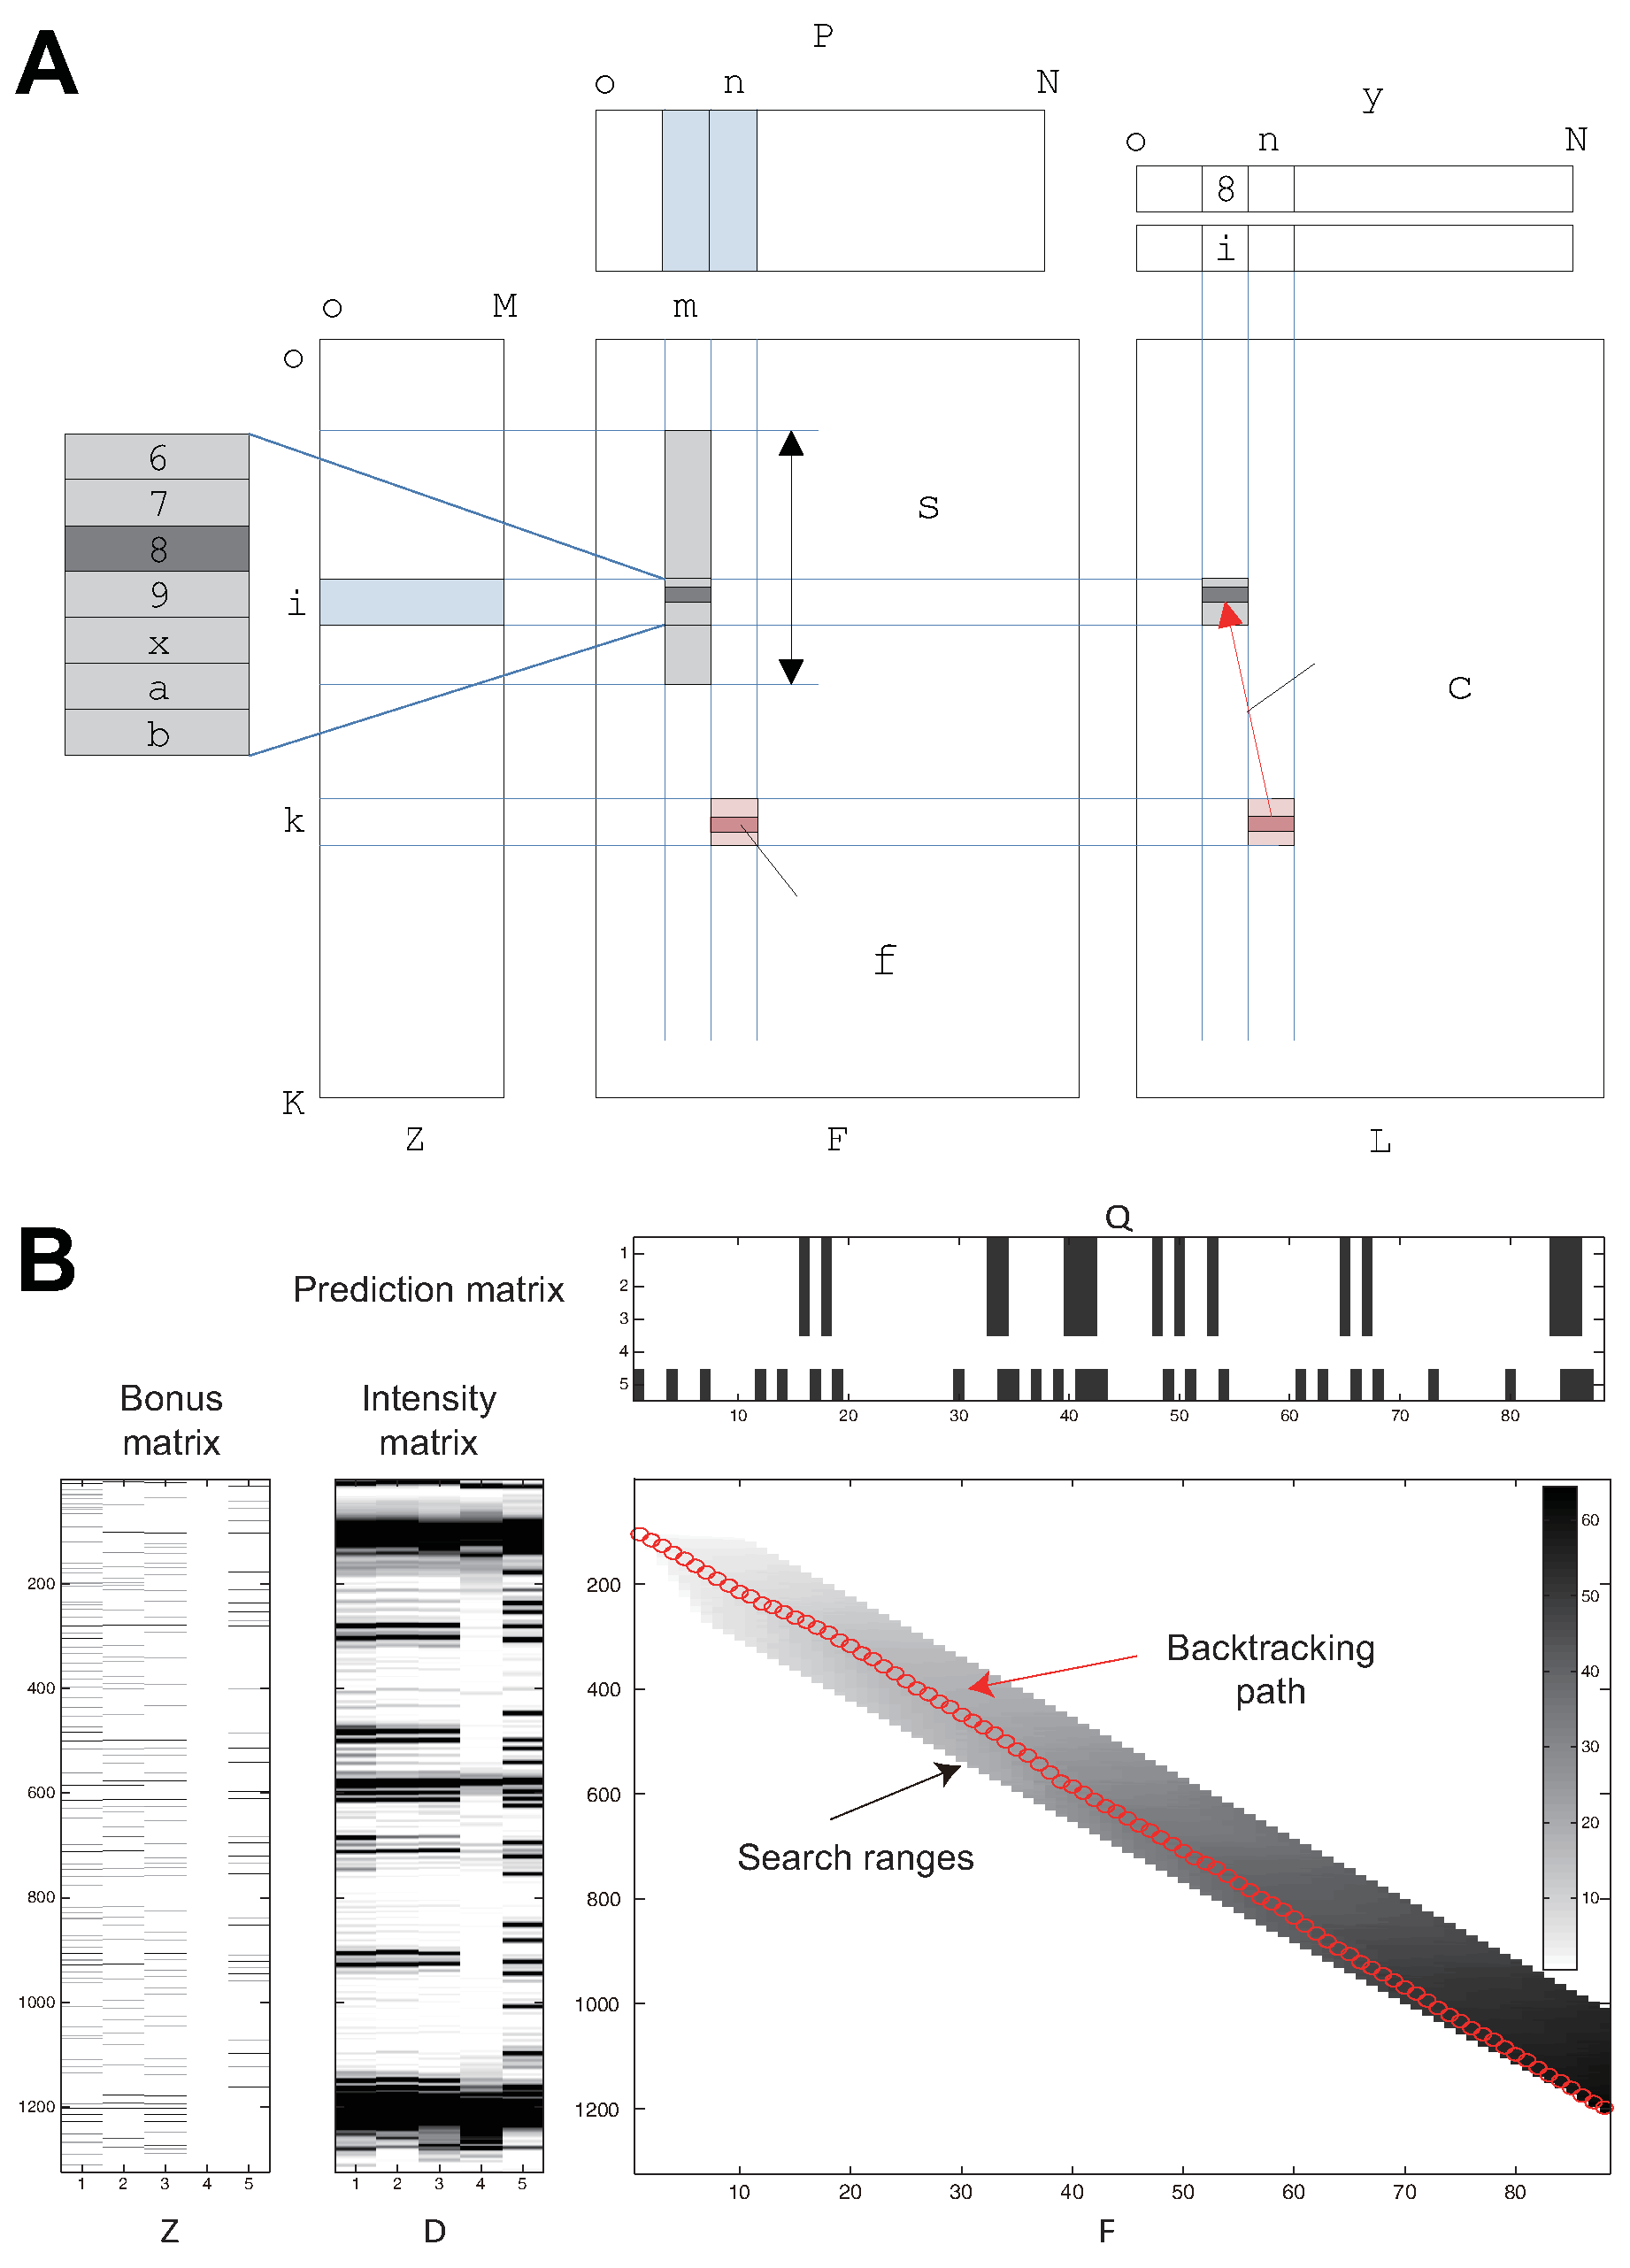
\includegraphics[width=0.85\linewidth]{figures/method_dp_formulation}
\caption{Formulation as dynamic programming. (\textbf{a}) $\bF(n,k,p)$ depends on $\bF(n-1,k',p')$ in the previous column and the gap bonus \hilight{$S(n,k',k,p)$} between them. The best tuple $(k',p')$ that maximizes $\bF(n,k,p)$ is searched for in the range $k-2.5\rho \le k' < k; k'+p' < k+p$ and is stored in the backtracking matrices $\bL_k(n,k,p)$, $\bL_p(n,k,p)$. The computation of $S(n,k',k,p)$ is based on the bonus matrix $\bB$ and the prediction matrix $\bP$ (Section~\ref{ss:cost}). (\textbf{b}) Example. The data set used is `FMN Apatamer with single binding site.' $N=88$, $M=5$, $K=1324$. The backtracking path is represented by a series of red circles superimposed on the score matrix $\bF$; since $\bF$ is 3-dimensional, the figure alternatively represents a reduced matrix $\bF'$ defined by $\bF'(n,k)=\max_{p'} \bF(n,k,p')$. The output array $\by_k$, which stores the position of each circle, indicates the band locations.}
\label{f:dp-formulation}
\end{figure}
%%%%%%%%%%%%%%%%%%%%%%%%%%%%%%%%%%%%%%%%%%%%%%%%%%%%%%%%%%%%%%%%%%%%%%%%%%%%%%%%


\subsection{Description of score term}\label{ss:cost}
The score term in (\ref{e:F2}) consists of the following two components:
%
\begin{equation}\label{e:score-term}
S(n,k',k,p) = S_{\textrm{dist}}(n,k-k') + w_{\textrm{peak}} \cdot \bold{S}_{\textrm{peak}} (k,p) \cdot \bC(n, :)
\end{equation}
%
where \hilight{$S_\textrm{dist}$ and $\bold{S}_\textrm{peak}$ are functions returning vectors of nonnegative elements}, and $\bC(n,:)$ is the $n$-th row of the prediction matrix $\bC$. The dot product in the second term is a sum over all lanes $m$ from 1 to $M$. \hilight{A coefficient $w_{\textrm{peak}}$ of 1.0 gave acceptable annotations in initial tests and was not further optimized.}


\subsubsection{Distance bonus term}

It is empirically supported that the length between consecutive locations, $k'$ and $k$, is quite evenly distributed. $S_{\textrm{dist}}$ is the bonus term that utilizes this fact and induces the dynamic programming to end up with regularly stretched output. In addition, observations on reference annotations suggest that a gap between two consecutive locations tends to be shorter when the preceding location corresponds to `$\mathtt{G}$' in the RNA sequence~\citep{mills1979structure,sasaki1998identification}. These observations lead to the definition of distance bonus term as follows:
%
\begin{equation}
S_{\textrm{dist}} (n,d) = {{f_{(\rho', {\rho \over 2})}(d)} \over {f_{(\rho', {\rho \over 2})}(\hilight{\rho'})}}
\end{equation}
%
where
%
\begin{equation}\nonumber
\rho' = \left\{
  \begin{array}{ll}
    {2 \over 3}\rho, &\hbox{if $\bs(n-1)=\mathtt{G}$;} \\
    \rho, &\hbox{otherwise}
  \end{array}
\right.
\end{equation}
%
and $f_{(\mu, \sigma)}$ is the density function of $N(\mu, \sigma)$. That is, $S_{\textrm{dist}}(n,d)$ reaches its maximum value 1 when $d = \rho'$ and decreases along a Gaussian curve as $d$ deviates from $\rho'$.

\subsubsection{Peak bonus term}\label{sss:peak_bonus_term}
The second score term favors band locations near peaks of the electrophoretic profiles with a significant curvature. As the peak bonus is granted only for the profiles with a band at the location, $\bC(n,:)$ must be referred before actually adding up the bonuses as demonstrated in the equation (\ref{e:score-term}).
$\bold{S}_{\textrm{peak}}$ is a function that returns a nonnegative $M$-dimensional value where each of its entries represents the peak bonus from each profile:
%
\begin{equation}
\bold{S}_{\textrm{peak}}(k,p) = (S^1_{\textrm{peak}}(k), \ldots, S^{M-1}_{\textrm{peak}}(k), S^M_{\textrm{peak}}(k,p))
\end{equation}
%
where $S^m_{\textrm{peak}}$ stands for the bonus from matching a peak to a band in $\ba_m$, assuming such a band exists. \hilight{The bonus was designed to be boosted for a greater curvature} at the peak and the proximity of the peak to the band, so $S^m_{\textrm{peak}}$ is defined as the product of a Gaussian density function and an entry of $\bB$ corresponding to the candidate peak closest to location $k$:
%
\begin{equation}
S^m_{\textrm{peak}}(k) = \max_{\substack{|q| < \rho/2}} {{f_{(0, {\rho \over 5})}(q)} \over {f_{(0, {\rho \over 5})}(0)}} \cdot \bB(k+q, m)
\end{equation}
%
for $m < M$, and
%
\begin{equation}\label{e:peak-matching}
S^M_{\textrm{peak}}(k,p) = {{f_{(0, {\rho \over 5})}(p)} \over {f_{(0, {\rho \over 5})}(0)}} \cdot \bB(k+p, m) \cdot (M-1)
\end{equation}
%
As described above, this peak bonus is taken from the primary profile (typically a sequencing ladder) rather than searching for optimal peak/band matches across all profiles to allow degeneracy breaking at reasonable computational expense. [A separate dynamic-programming-based band annotation algorithm was also tested which does not carry out the peak/band degeneracy breaking of eq. (\ref{e:peak-matching}) and gave slightly worse performance; see Supplemental Figure S2.]


\subsection{Reliability evaluation}\label{ss:reliability-evaluation}
While the presented band annotation method was found to be quite accurate, it was not perfect. We therefore sought a method to assess the reliability of automatically determined band locations prior to practical application. We devised a score to predict the quality of results. The idea behind the score is that when optimization of eq. (\ref{e:score-term}) fails to achieve the desirable solution, we typically see extraordinarily short or long distances between consecutive locations (little information from $S_\textrm{dist}$) or bands on the primary profile without proper matching to peaks (little information from $S_\textrm{peak}$). The $\escore$-score is defined with the following terms:
\begin{itemize}
\item $n_1$: number of bands on the primary profile without corresponding peak
\item $n_2$: number of gaps with length less than $\rho/4$, or greater than $2\rho$
\item $N^\textrm{peak}_M$: number of bands on the primary profile predicted by $\bC$
\item $\escore = 1 - {\max({{n_1} \over N^\textrm{peak}_M}, {{n_2} \over {K-1}})}$
\end{itemize}
$\escore$-score is a value between 0 and 1 and conservatively estimates the number of normalities in the output relative to the number of bands and locations. Greater $\escore$-score means less abnormalities in the output which is believed to result from output digressing from the correct answer, so it can be expected that output with $\escore$ closer to 1 would be more reliable than output with smaller $\escore$. The relationship between $\escore$-score and accuracy is presented in the Results section.

\begin{comment}
\subsection{Implementation}
We implemented the proposed method in the MATLAB programming environment (The MathWorks, http://www.mathworks.com) and are making it freely available for download at http://hitrace.stanford.edu.
(To be filled with data preparation...)
\end{comment}

%%%%%%%%%%%%%%%%%%%%%%%%%%%%%%%%%%%%%%%%%%%%%%%%%%%%%%%%%%%%%%%%%%%%%%%%%%%%%%%
% TABLE 1
%%%%%%%%%%%%%%%%%%%%%%%%%%%%%%%%%%%%%%%%%%%%%%%%%%%%%%%%%%%%%%%%%%%%%%%%%%%%%%%
\begin{table}
\processtable{High-throughput RNA structure mapping data sets analyzed by the proposed method (total 522 profiles and 47210 bands). Excluding the last line, there are 95 data sets. More details of these 95 data sets are described in \citet{lee2014eterna}. %The last data set is from a study on a 187-nt ribozyme.
\label{t:data}}
{\begin{tabular}{lcccc}
\toprule
Name& \# profiles & \# nt & \# bands per profile & \# total bands \\
\midrule
R45$^a$  &60&	108&	88&	5280\\
R46$^a$  &80&	108&	88&	7040\\
R47$^b$  &90&	112&	92&	8280\\
R47B$^b$  &36&	112&	92&	3312\\
R48$^b$  &96&	112&	92&	8832\\
R49$^b$  &18&	112&	92&	1656\\
R49B$^c$  &48&	115&	95&	4560\\
R50$^c$  &54&	115&	95&	5130\\
R43$^d$  &40&	98&	78&	3120\\
%HDV$^e$ & 4& 187 & 187 & 748\\
\botrule
\end{tabular}}
{$^a$Flavin mononucleotide (FMN) aptamer with single binding site~\citep{lee2014eterna}; $^b$FMN aptamer with single binding site II; $^c$FMN binding branches; $^d$The backwards C%; $^e$NMIA (SHAPE) modification of the hepatitis delta virus (HDV) ribozyme
%Abbreviations: FMN, flavin mononucleotide
}
%Abbreviations: SRP, signal recognition particle conserved domain; P4-P6, P4-P6 domain of the Tetrahymena group I ribozyme; DMS, dimethyl sulfate; CMCT, 1-cyclohexyl-3-(2-morpholinoethyl) carbodiimide metho-p-toluenesulfonate; SHAPE, selective hydroxyl acylation analyzed by primer extension.}
\end{table}



